% This must be in the first 5 lines to tell arXiv to use pdfLaTeX, which is strongly recommended.
\pdfoutput=1
% In particular, the hyperref package requires pdfLaTeX in order to break URLs across lines.

\documentclass[11pt]{article}

% Remove the "review" option to generate the final version.
\usepackage[review]{emnlp2021}

% Standard package includes
\usepackage{times}
\usepackage{latexsym}

% For proper rendering and hyphenation of words containing Latin characters (including in bib files)
\usepackage[T1]{fontenc}
% For Vietnamese characters
% \usepackage[T5]{fontenc}
% See https://www.latex-project.org/help/documentation/encguide.pdf for other character sets

% This assumes your files are encoded as UTF8
\usepackage[utf8]{inputenc}
\renewcommand{\UrlFont}{\ttfamily\small}
\usepackage{graphicx}
\usepackage{grffile}
\usepackage{multirow}
\usepackage{xcolor,colortbl}
\usepackage{amsmath}
%\usepackage{fdsymbol}
\usepackage{amssymb}
\usepackage{makecell}
\usepackage[super]{nth}
\usepackage{arydshln}

\usepackage{algorithm}
\usepackage[noend]{algpseudocode}
\usepackage{regexpatch}
\usepackage{subcaption}
% This is not strictly necessary, and may be commented out,
% but it will improve the layout of the manuscript,
% and will typically save some space.
\usepackage{microtype}

\usepackage{url}
\usepackage{longtable}
\usepackage{tikz}
\usetikzlibrary{calc}
\usepackage[draft]{todo}
\usepackage[normalem]{ulem}
\usepackage{xspace}
\usepackage{float}

\usepackage{pgfplots}
\usepackage{pgfplotstable}

\let\oldbibitem\bibitem
\def\bibitem{\vfill\oldbibitem}

\usepackage{soulutf8}
\usepackage{tabularx}

\usepackage{multirow}
\usepackage{adjustbox}
\usepackage{caption}
\usepackage{subcaption}

\newcommand{\fyTodo}[1]{\Todo[FY:]{\textcolor{orange}{#1}}}
\newcommand{\fyTodostar}[1]{\Todo*[FY:]{\textcolor{orange}{#1}}}
\newcommand{\fyDone}[1]{\done[FY]\Todo[FY:]{\textcolor{orange}{#1}}}
\newcommand{\fyFuture}[1]{\done[FY]\Todo[FY:]{\textcolor{red}{#1}}}
\newcommand{\fyDonestar}[1]{\done[FY]\Todo[FY:]{\textcolor{orange}{#1}}}

\newcommand{\revision}[1]{\textcolor{red}{#1}}
\newcommand{\revisiondel}[1]{}
\newcommand{\src}{\ensuremath{\mathbf{f}}} % source sentence
\newcommand{\trg}{\ensuremath{\mathbf{e}}} % target sentence
\newcommand{\domain}[1]{\texttt{\textsc{#1}}}
\newcommand{\system}[1]{\texttt{{#1}}}

\newcommand{\vlambda}{\ensuremath{\boldsymbol\lambda}\xspace} % parameters vector for a distribution
\newcommand{\vtheta}{\ensuremath{\boldsymbol\theta}\xspace} % parameters vector for a distribution
\newcommand{\vpsi}{\ensuremath{\boldsymbol\psi}\xspace} % parameters vector for a distribution
\newcommand{\indic}[1]{\ensuremath{\mathbb{I}(#1)}}
% \newcommand{\SB}[1]{\textcolor{green}{#1}}
% \newcommand{\SW}[1]{\textcolor{red}{#1}}
\newcommand{\SB}[1]{\textbf{#1}}
\newcommand{\SW}[1]{\underline{#1}}
% limits underneath
\DeclareMathOperator*{\argmin}{arg\,min}
\DeclareMathOperator*{\argmax}{arg\,max}
\renewcommand\textfraction{.1}
\renewcommand\floatpagefraction{.95}
\newcommand{\sbcl}[2]{{\scriptsize #1 \hfill $|$ \hfill  #2}}
\usepackage{multirow}
\usepackage{adjustbox}

\title{Multi-Domain Adaptation in Neural Machine Translation with Dynamic Sampling Strategies}

\author{First Author \\
  Affiliation / Address line 1 \\
  Affiliation / Address line 2 \\
  Affiliation / Address line 3 \\
  \texttt{email@domain} \\\And
  Second Author \\
  Affiliation / Address line 1 \\
  Affiliation / Address line 2 \\
  Affiliation / Address line 3 \\
  \texttt{email@domain} \\}

\date{}

\begin{document}
\maketitle
\setlength{\abovedisplayskip}{2pt}
\setlength{\belowdisplayskip}{2pt}
\begin{abstract}
  Building effective Neural Machine Translation models often imply accommodating diverse sets of heterogeneous data so as to optimize performance for the domain(s) of interest. Such multi-source / multi-domain adaptation problems are typically approached through instance selection or reweighting strategies, based on a static assessment of the relevance of training instances with respect to the task at hand. In this paper, we study dynamic data selection strategies that are able to automatically re-evaluate the usefulness of data samples and to evolve a data selection policy in the course of training. Based on the results of multiple experiments, we show that such methods constitute a generic framework to automatically and effectively cater to a variety of real-world situations, from supervised multi-source domain adaptation to multi-domain learning and unsupervised domain adaptation. 
\end{abstract}

\section{Introduction}\label{sec:intro}
A typical setting in machine translation (MT) is to collect the largest possible collection of parallel data for the chosen language pair, with the intent to achieve optimal performance for a task of interest. In such situations, the training data distribution is opportunistic, while the test data distribution is chosen and fixed; a key component in training is then to mitigate the detrimental effects of a possible mismatch between these distributions. Single-source and multi-source domain adaptation (DA) is a well-studied instance of this setting (see \citet{Chu2017comparison} for a review), and so is multi-domain (MD) learning \citep{Chu18multilingual,Zeng18multidomain,Jiang19multidomain,Pham21revisiting}. A related situation is multilingual machine translation \citep{Firat16multiway,Ha16towards,Johnson17google,Arivazhagan19massively}\fyTodo{Add more recent work}, where the heterogeneity of training data not only corresponds to variations in topic, genre or register, but also in language.

This problem is often approached by \emph{static} instance selection or re-weighting strategies, where the available training data is used in proportion to its relevance for the chosen test conditions \citep{Moore10selection,Axelrod11domain}. Finding the optimal balance of training data is however a challenging task due, for instance, to the similarity between domains/languages, but also due to regularization effects of out-of-domain data; it may also be suboptimal, as some target domains or languages might be easier to train than others. For example, improving the performance of the MT system in one domain will often hurt that of another \citep{Vanderwees17dynamic, Britz17mixing}, and improving model generalization across all domains \citep{koehn18findings} may not promise optimization of a particular domain. 

Several recent proposals \citep{platanios19competence,Zhang19curriculum,Kumar19reinforcement,Wang20learning-multi,Graves17automated,Wang20balancing,Wang20learning-multi,Vanderwees17dynamic} have explored ways to instead consider \emph{dynamic} data selection and sampling strategies that surpass static strategies. Furthermore \citet{Zhang19curriculum,Vanderwees17dynamic} construct a static curriculum while \citet{platanios19competence,Kumar19reinforcement,Graves17automated,Wang20balancing,Wang20learning-multi} build curricula automatically adapted to the training.

In this paper, we propose a novel method of building an automated curriculum for training the Multi-Domain NMT model, that is inspired by the work of \citet{Graves17automated}. We evaluate our method in various single-domain and multi-domain adaptation settings. We compare our method with several contrasts including the work of \citet{Zhang19curriculum} and \citet{Wang20balancing}. From now on, we name our method MDAC which is brief for Multi-Domain Automated Curriculum. Based on experimental results obtained on a diverse set of domains, our main conclusions are that (a) using MDAC often yields overall performance that are as good as the standard fine-tuning strategy for domain adaptation; (b) MDAC can effectively handle a variety of test target distributions.

\section{Learning with multiple data sources} \label{sec:mdmt}

We conventionally define a domain $d$ as a distribution $\mathcal{D}_d(x)$ over some feature space $\mathcal{X}$ that is shared across domains \citep{Pan10asurvey}: in machine translation, $\mathcal{X}$ is the representation space for input sentences; each domain corresponds to a specific source of data, and may differ from the other data sources in terms of textual genre, thematic content \cite{Chen16guided,Zhang16topicinformed}, register \cite{Sennrich16politeness}, style \cite{Niu18multitask}, etc. Translation in domain $d$ is formalized by a translation function $h_d(y|x)$ pairing sentences in a source language with sentences in a target language $y \in \mathcal{Y}$. $h_d$ is usually assumed to be deterministic (hence $y = h_d(x)$), but might differ from one domain to the other.

It is usual in MT to opportunistically collect training samples from several domains, which means that training instances are distributed according to the mixture $\mathcal{D}^s$ such that $\mathcal{D}^s(x) = \sum_{d=1}^{n_d} \lambda^{s}(d) \mathcal{D}_d(x)$, where $\{\lambda^{s}(d), d=1 \dots n_d\}$ are the corresponding mixture weights satisfying $\sum_d \lambda^{s}(d)=1$.

The main challenge is then to make the best of this heterogeneous data, with the aim to achieve the optimal performance for the intended test conditions. These might correspond to data from just one of the training domains, as in standard supervised (multi-source) domain adaptation; a more difficult case is when the test data is from one domain unseen in training (unsupervised domain adaptation); in multi-domain adaptation finally, the test distribution is itself a mixture of domains, some of which may also be observed in training.  Without loss of generality, one may then assume that the test distribution takes the form $\mathcal{D}^{t}(x) = \sum_d \lambda^{t}(d) \mathcal{D}_d(x)$ - with only one non-null  component in the case of fine-tuning.
These situations are illustrated in Figure~\ref{fig:mdmt-lambdas}.
\begin{figure}[h]
  \centering
  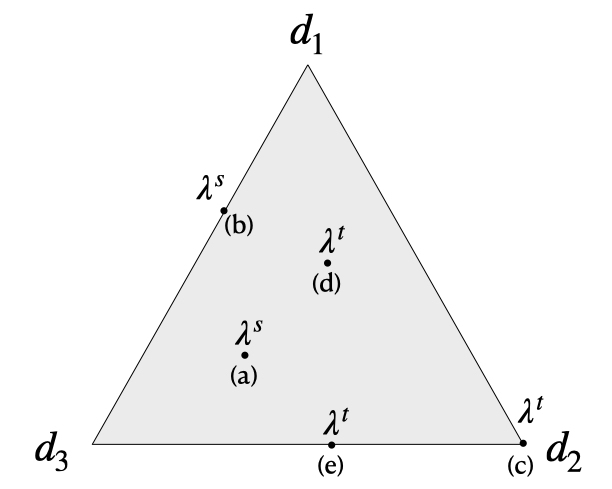
\includegraphics[width=0.48\textwidth]{mdmt-lambdas}
  \caption{Training and testing with distribution mismatch. We consider just three domains, and represent vectors of mixture weights $\vlambda^{s}$ and $\vlambda^{t}$ in the 3-dimensional simplex. Training with weights in (a) and testing with weights in (c) is supervised multi-source domain adaptation to domain~2 ($d_2$), while (b)-(c) is the unsupervised version, with no training data from $d_2$; training with weights in (a) and testing with weights in (d) is multi-domain learning, also illustrated with configurations (a)-(e) (training domain $d_1$ is not seen in test), and (b)-(d)  (test domain $d_2$ is unseen in training).}\label{fig:mdmt-lambdas}
\end{figure}

These situations have been amply documented from a theoretical perspective (eg.\ \cite{Mansour09multiple,Mansour09domainadaptation,Hoffman18algorithms}). A general recommendation in the DA setting is to adjust the sampling distribution used to optimize the system so as to compensate for the mismatch between $\mathcal{D}^s(x)$ and $\mathcal{D}^t(x)$. This can be approximated by reweighting instances, or more conveniently domains, which are selected during training with a probability $\lambda^{l}(d)$, with $\lambda^{l}(d) \neq \lambda^{s}(d)$.

A more practical standard approach to supervised DA is \emph{fine-tuning} \cite{Luong15stanford,Freitag16fast}, where $\vlambda^{l}$ is allowed to vary during learning. With our notations, this approach amounts to first learning an initial parameter value with all the data ($\forall d, \lambda^{l}(d) = \lambda^{s}(d)$), then to continue training with only batches from the test domain $d_t$ ($\lambda^{l}(d) = \indic{d = d_t}$) with $\indic{A}$ the indicator function for predicate $A$. Note that this strategy is potentially suboptimal, as some out-of-domain samples may contribute to the final performance due to eg.\ domain overlap. Optimizing the learning distribution in multi-domain settings is even more challenging, as the learner has to best take advantage of potential domains overlaps, and also of the fact that some domains might be easier to learn than others.\fyTodo{How to measure this?} \revision{Answer: The graphic of \system{Mixed-0} shows that with the same amount of data(batches) the convergences of the domains vary significantly}

% === The part on multidomain training has been moved to the end.

\section{Multi-Domain Automated Curriculum } \label{sec:mdac}
\subsection{Basic principles}
Assuming training data from $n_d$ domains $d_1 \dots d_{n_d}$, we denote the size of the training corpus from domain $d$ as  $N^{s}_d$, and $N^{s} = \sum_d N^{s}_d$ is the total number of training samples. We use $\widehat{\mathcal{D}^l_d}$ and $\widehat{\mathcal{D}^t _d}$ to denote the empirical train and test distributions for domain $d$, and $\widehat{\mathcal{D}^{u}}(x;\lambda^{u}) = \sum_{d} \lambda^{u}(d) \widehat{\mathcal{D}^{u}_d}(x)$ for $u\in\{l,t\}$. In our setting,  $\vlambda^t$, and hence $\widehat{\mathcal{D}^t}(x;\vlambda^t)$ are fixed and predefined, approximated with an equivalent number of development corpora. 

Our method MDAC constructs an automatically adapting distribution $\lambda^{l}$ that optimizes the data selection policy along with the training of the NMT model. We parameterize $\lambda^{l}$ by a differentiable function $\lambda^l(\psi)$. We divide the training into many short sessions; in each session $t$, the model is trained with a static data distribution $\lambda^{l}(\psi_t)$. After one learning session, we update the data distribution via REINFORCE algorithm \citep{Williams92simple}.

\begin{align*}
\psi_{t+1} &= \psi_t + \mathbf{lr}_{1} * \displaystyle{\mathop{\sum}_{d=1}^{n_d}} R(d) * \frac{\partial \lambda^l(d;\psi_t)}{\partial \psi} \\
\end{align*}
\begingroup
\allowdisplaybreaks
With the following reward computation:
\begin{align*}
  R(d) = J^t(\theta_{t+k},\vlambda^t) - J^t(\theta_t,\vlambda^t)
\end{align*}
Where 
\begin{equation}
\begin{array}{rcl}
\theta_{t+i} &=& Update\big(\theta_{t+i-1},[x^i_j,y^i_j]_{j=1}^N\big) \\ \nonumber
x^i_j, y^i_j &\sim& \widehat{D^l_d}(x) \\
J^t(\theta,\lambda_t) &=& \displaystyle{\mathop{\sum}_{d=1}^{n_d}}\lambda^t(d)\displaystyle{\mathop{\sum}_{x^t_d,y^t_d \in \widehat{D^t_d}}} l(\theta,x^t_d,y^t_d)
\end{array}
\end{equation}
\endgroup
%\theta_{t+i-1} - \mathbf{lr_2} \frac{1}{N}\displaystyle{\mathop{\sum}_{j=1}^N}\frac{\partial l(\theta_{t+i-1}, x^i_j,y^i_j)}{\partial \theta}
$N$ is the size of a batch; $\mathbf{lr}_{1}$ is the learning rate of the sampling distribution; $\mathbf{lr_2}$ is the learning rate of the NMT system; $l(\theta,x,y)$ is the loss of the NMT model on the sample $(x,y)$; $J^t(\theta,\lambda_t)$ is the weighted loss computed over $n_d$ dev-sets corresponding to $n_d$ given domains.

To compute the reward of using data from domain $d$ to train the model, $R(d)$, we simulate $k$ training steps from the current checkpoint by training the model with k batches sampled from $D^l(d)$ and compute the gain of the weighted dev-loss. The reward of our method is inspired by the target prediction gain in \cite{Graves17automated}. However, \cite{Graves17automated} used accumulated gains from the past as reward while we use the "future" gain as reward. Furthermore, the choice of the parameterization of the sampling distribution in our method is different from one in \cite{Graves17automated}, although this choice is empirical.

The work of \cite{Wang20balancing} based on the Bi-level Optimization framework, which aims to find an optimal static distribution $\lambda^{l}$ that will result in the best NMT model regarding a given target dev set at the end of the training, derives also a similar form of update for $\psi$. However, their reward is the cosine similarity between the gradient computed with the training data and the gradient computed with the dev set.

\subsection{MDAC for (multi) domain adaptation}
This setting is pretty general and can in principle accommodate the variety of situations mentioned  above, and many more: basic domain adaption, multi-domain adaptation with various target distributions, possibly including domains unseen in training. In our experiments we would like to better assess the actual potential of MDAC is these settings and seek to experimentally answer the following questions:
\begin{itemize}
\item is MDAC a viable alternative to conventional fine-tuning? In particular does it enable to better take advantage of relevant data from other domains?
\item is MDAC also a viable option in multi-domain adaptation scenarios?
\item does MDAC also enable to perform unsupervised (multi-) domain adaptation? \fyDone{TBContinued}
\end{itemize}

These questions are further explored in Section~\ref{sec:results}. We now turn to our experimental conditions.

\section{Experimental settings} \label{sec:exp}
\subsection{Data and metrics \label{ssec:corpora}}
We experiment with translation from English into French and use texts initially originating from 6~domains, corresponding to the following data sources: the UFAL Medical corpus V1.0 (\domain{med})\footnote{\url{https://ufal.mff.cuni.cz/ufal_medical_corpus}. We only use the in-domain (medical) subcorpora: PATR, EMEA, CESTA, ECDC.}; the European Central Bank corpus (\domain{bank}) \cite{Tiedemann12parallel}; the JRC-Acquis Communautaire corpus (\domain{law}) \cite{Steinberger06acquis}; documentations for KDE, Ubuntu, GNOME and PHP from the Opus collection \cite{Tiedemann09news}, merged in a \domain{it}-domain; TedTalks (\domain{talk}) \cite{Cettolo12wit}, and the Koran (\domain{rel}). Complementary experiments also use v12 of the News Commentary corpus (\domain{news}). Most corpora are available from the Opus website.\footnote{\url{http://opus.nlpl.eu}} These corpora were deduplicated and tokenized with in-house tools; statistics are in Table~\ref{tab:Corpora}. To reduce the number of types and build open-vocabulary systems, we use Byte-Pair Encoding \cite{Sennrich16BPE} with 30,000 merge operations on a corpus containing all sentences in both languages.\fyDone{Add \# number of tokens, also specificity ?}%

We randomly select in each corpus a development and a test set of 1,000 lines and keep the rest for training. Validation sets are used to chose the best model according to the average BLEU score \cite{Papineni02bleu}.\footnote{We use truecasing and the \texttt{multibleu} script.}\fyDone{A word about meta-parameter settings} Significance testing is performed using bootstrap resampling \cite{Koehn04statistical}, implemented in compare-mt\footnote{\url{https://github.com/neulab/compare-mt}} \cite{Neubig19compare-mt}. We report significant differences at the level of $p=0.05$.\fyDone{Fix correct p value}

\begin{table*}[htbp]
  \centering
  \begin{tabular}{|l|ccccccc|} %*{4}{|r|}}
    \cline{2-8} 
    %\multicolumn{4}{|l|}{Vocab size - En: 30,165, Fr: 30,398}\\
    \multicolumn{1}{c|}{} & \multicolumn{1}{c}{\domain{med}} & \multicolumn{1}{c}{\domain{law}} & \multicolumn{1}{c}{\domain{bank}} & \multicolumn{1}{c}{\domain{it}} & \multicolumn{1}{c}{\domain{talk}} & \multicolumn{1}{c}{\domain{rel}} & \multicolumn{1}{c|}{\domain{news}} \\
    \hline 
    \# lines & 2609 (0.68) & 501 (0.13) & 190 (0.05) & 270 (0.07) & 160 (0.04) & 130 (0.03) & 260 (0) \\
    \# tokens &  133 / 154  &  17.1 / 19.6 &  6.3 / 7.3 &  3.6 / 4.6 &  3.6 / 4.0 &  3.2 / 3.4 & 7.8 / 9.2   \\
    \# types & 771 / 720 & 52.7 / 63.1 & 92.3 / 94.7 & 75.8 / 91.4 & 61.5 / 73.3 & 22.4 / 10.5 & - \\
    \# uniq & 700 / 640 & 20.2 / 23.7 & 42.9 / 40.1 & 44.7 / 55.7 & 20.7 / 25.6 & 7.1 / 2.1 & - \\
    \hline
  \end{tabular}
  \caption{Corpora statistics: number of parallel lines ($\times 10^3$) and proportion in the training domain mixture (which does not contain \domain{news}), number English and French tokens ($\times 10^6$), number English and French types ($\times 10^3$), number of types that only appear in a given domain ($\times 10^3$). \domain{med} is the largest domain, containing almost 70\% of the sentences, while \domain{rel} is the smallest, with only 3\% of the data.
  }
\label{tab:Corpora}
\end{table*}

\subsection{Baseline systems \label{ssec:baseline}}
Our baselines are standard for multi-domain systems.\footnote{We however omit domain-specific systems trained only with the corresponding subset of the data, which are always inferior to the mix-domain strategy \cite{Britz17mixing}.} Using Transformers \cite{Vaswani17attention} implemented in OpenNMT-tf\footnote{\url{https://github.com/OpenNMT/OpenNMT-tf}} \cite{Klein17opennmt}, we build the following systems:

\begin{itemize}
\itemsep0em 
\item Generic models trained with various predefined mixtures of the training data taking the form:
\begin{align} \label{mixture:trn}
\lambda_{\alpha}(d) = \frac{q_d^{\alpha}}{\displaystyle{\mathop{\sum}_{d=1}^{n_d}q_d^{\alpha}}} &&
q_d = \frac{\mid N^{s}_d \mid}{\displaystyle{N^{s}}} % \mathop{\sum}_{i=1}^K\mid D_i \mid}}
\end{align} \setlength{\abovedisplayskip}{2pt}
\setlength{\belowdisplayskip}{2pt} 
with $\alpha \in [0,0.25,0.5,0.75,1.0]$. These systems are denoted \system{Mixed-$\alpha$} below. \system{Mixed-$0$} uses a uniform domain distribution, \system{Mixed-$1.0$} uses the observed domain distribution.
\item fine-tuned models \cite{Luong15stanford,Freitag16fast}, based on the \system{Mixed-$1.0$} system, further trained on each domain for at most 50~000 iterations, with early stopping when the dev BLEU stops increasing. The full fine-tuning (\system{FT-Full}) procedure may update all the parameters of the initial generic model, resulting in six systems each adapted for one domain, with no parameter sharing across domains.
 
\item Our comparison of multi-domain systems includes baselines with fixed data mixtures corresponding to $\lambda^l \in \big[ \lambda_0, \lambda_{0.25}, \lambda_{0.5}, \lambda_{0.75}, \lambda_{1.0}\big]$, and our reimplementations of recent proposals from the literature: Curriculum Learning of \cite{Zhang19curriculum} that we denote CL and Differential Data Selection of \cite{Wang20balancing} that we denote DDS.
\end{itemize}

All models use embeddings and hidden layers sizes of dimension~512. Transformer models contain 8~attention heads in each of the 6+6 layers; the inner feedforward layer contains 2048 cells. The adapter-based systems (see below) additionally use an adaptation block in each layer, composed of a 2-layer perceptron, with an inner $\operatorname{ReLU}$ activation function operating on normalized entries of dimension~1024. 
Training uses batches of~12,288 tokens, Adam with parameters $\beta_1=0.9$, $\beta_2= 0.98$, Noam decay ($warmup\_steps=4000$), and a dropout rate of $0.1$ in all layers.

\subsection{MDAC systems} \label{ssec:dds-sys}
The behavior of MDAC only depends on (a) the initial domain distribution at the start of training $\vlambda^{l}_{t=0}$, and (b) the targeted (dev/test) distribution $\vlambda^{t}$. We will thus report these systems as \system{MDAC($\vlambda^{l}_{t=0}$, $\vlambda^{t}$)}. We also compare our method with the method DDS under the same conditions.

In our work, we simply parameterize the distribution $\lambda^l$ as follows.
\begin{equation}
\lambda
^l(d;\vpsi) = \frac{\vpsi[d]^\beta}{\sum_i \vpsi[i]^\beta} \nonumber
\end{equation}
We choose $\beta=2$ for our experiments.

We also provide in this section our choices of the hyper-parameters of our algorithm including the number of simulation training steps $k=10$, and the update rate $\mathbf{lr}_{data}=0.1$. We split the training into many short sessions that last 2000 training steps each.
\subsection{CL and DDS's re-implementation}
We re-implement DDS in Tensorflow without any change in the choices of parameterization and hyper-parameters compared to original code of \citet{Wang20balancing} \footnote{\url{https://github.com/cindyxinyiwang/multiDDS}}.

We re-implement the work of \citet{Zhang19curriculum} by following exactly the description of the algorithm. For each experiment of adapting the NMT system to one domain, we combine the training data of other domains into one corpus, then compute the cross-entropy difference score of each sentence of this corpus (we only compute the score for the source side). We sort and split the corpus into 9 shards and execute curriculum learning with 10 shards in which the first shard is the in-domain corpus.
\subsection{Experimental tasks}
We evaluate the efficacy of our methods compared to several aforementioned baselines via 5 tasks including domain adaptation; multi-domain adaptation, bi-domain adaptation, unseen domain adaptation, and unsupervised domain adaptation.

In the domain adaptation task, given the data of 6 domains including \domain{med}, \domain{bank}, \domain{law}, \domain{it}, \domain{talk}, \domain{rel}, we aim to build expert NMT models for each domain respectively.

In the multi-domain adaptation task, given the data of 6 domains, we aim to build an NMT model which gives the best performance regarding a predefined test set containing equivalently 6 domains.

In the bi-domain adaptation task, given the data of 6 domains, we only focus on 2 domains of them.

In the fourth experiment, given the data of 6 domains and a small dev set of an unseen domain, which is News, in this case, we aim to build an NMT model which is robust to the unseen domain.

In the unsupervised domain adaptation task, we cluster the training data of 6 domains into 30 clusters using the KNN algorithm in the same way as in the work of \citet{Tars18multidomain}, then adapt these clusters to one of 6 domains given the corresponding in-domain dev set. We compare MDAC to DDS over 6 domains.

\section{Results and discussion \label{sec:results}}

\subsection{Domain Adaptation}
In this setting, we aim to build an expert NMT model in only one domain. This setting corresponds to Dirac distribution $\lambda^t$, in which the probability of domains is 0 except for one domain.

We initialize MDAC and DDS by 2 different distribution $\lambda_0$ and $\lambda_1$. According to Table \ref{tab:da}, MDAC achieves the best performance with $\lambda_0$ initial where all domains have the same probability to be chosen. The same conclusion is also true for DDS.

According to Table \ref{tab:da}, MDAC is outperformed by fine-tuning method in large domains including \domain{med} and \domain{law}. However, MDAC improves fine-tuning by approximately 0.5 BLEU in \domain{bank} and 1.0 BLEU in \domain{rel}. This indicates that for small domains, out-of-domain data can improve the generalization of the NMT model and MDAC is capable to exploit this advantage by balancing the in-domain and the out-of-domain training data instead of edging out the out-of-domain training data as in fine-tuning.

DDS also demonstrates promising results in this task but is always outperformed by MDAC overall. The same conclusion is also applied to the CL method.

\begin{table*}[htbp]
  \centering \small
  \begin{tabular}{|l|*8{r|}} \hline
    domain \hfill $d=$ & \multicolumn{1}{c|}{\domain{ med}} & \multicolumn{1}{c|}{\domain{ law}} & \multicolumn{1}{c|}{\domain{bank}} & \multicolumn{1}{c|}{\domain{talk}} & \multicolumn{1}{c|}{\domain{ it }} & \multicolumn{1}{c|}{\domain{ rel}} & \multicolumn{1}{c|}{mean} \\ \hline
    FT-Full($d$) \hfill [BLEU] &37.7&59.2&54.5&34&46.8&90.8&53.8\\ \hline
    \hline
    \system{CL($d$)} &37.2&55.4&53.0&31.3&45.3&90.8&52.2\\ \hline
    \system{DDS($\vlambda_0, \vlambda_d$)} &36.7&56.2&54.3&33.5&46.8&91.8&53.2\\
    \system{MDAC($\vlambda_0, \vlambda_d$)} &36.7&58.2$^{**}$&55$^{*}$&33.3&46.6&91.9$^{***}$&53.6\\
     \hline
    \system{DDS($\vlambda_1, \vlambda_d$)} &36.4&56.3& 45.4& 32.6&44.5&43.1&43.1\\
    \system{MDAC($\vlambda_1, \vlambda_d$)} &37.2&55.1&51.8&32.8&44.9&85.4&51.2 \\ \hline
  \end{tabular}
  \caption{We report scores of each method with 6 target domains, and compare with full fine-tuning: each column corresponds to a distinct system. ($^{*}$) MDAC is significantly better than CL, fine-tuning and DDS with $p<0.05$. ($^{**}$) MDAC is significantly better than CL and DDS with $p<0.05$. ($^{***}$) MDAC is significantly better than CL, fine-tuning with $p<0.05$}
  \label{tab:da}
\end{table*}

\subsection{Multi-domain adaptation}

Multi-domain adaptation task requires best averaged performance of the NMT model in 6 domains. This setting corresponds to the uniform test distribution $\lambda^t = \lambda_0$. In this situation, the method CL of \citet{Zhang19curriculum} can not be applied. We therefore only compare the performance of MDAC, DDS and several fixed training data distribution $\lambda^l \in \big[ \lambda_0, \lambda_{0.25}, \lambda_{0.5}, \lambda_{0.75}, \lambda_{1.0}\big]$. The definition of those notations can be found in the equation \ref{mixture:trn}.

We initialize MDAC and DDS by 2 different distribution $\lambda_0$ and $\lambda_1$. According to Table \ref{tab:multi-da}, MDAC achieves the best performance with $\lambda_0$ initial where all domains have the same probability to be chosen. The same conclusion is also true for DDS.

MDAC outperforms static training distributions including $\big[ \lambda_0, \lambda_{0.75}, \lambda_{1.0}\big]$ with significant margin while performs slightly better than $\big[ \lambda_{0.25}, \lambda_{0.5} \big]$. This observation indicates that MDAC allows us to skip the heuristic choice for the training mixture of different domains or tasks.

The second observation is that DDS is again outperformed by MDAC with a significant margin of 0.5 BLEU on average. However, MDAC is surpassed by far with 1.8 BLEU in the domain \domain{med} by DDS. 

We show in the below figure \ref{fig:sampling}, the evolution of the training mixture through training sessions. According to the figure \ref{fig:DDS} of DDS, the proportion of 6 domains converges rapidly to bi-domain mode in which only \domain{med} and \domain{rel} have significant probability. In contrast, the proportion of 6 domains computed by MDAC evolves smoothly; small domains including \domain{bank}, \domain{it}, \domain{talk} and \domain{rel} take larger proportion in the beginning then decrease their proportions while larger domains as \domain{med} and \domain{law} increase their proportions in the end where the NMT model might have been already close to the optimal performance in the smaller domains.

\begin{table*}[htbp]
  \centering \small
  \begin{tabular}{|l|*8{r|}} \hline
    domain \hfill $d=$ & \multicolumn{1}{c|}{\domain{ med}} & \multicolumn{1}{c|}{\domain{ law}} & \multicolumn{1}{c|}{\domain{bank}} & \multicolumn{1}{c|}{\domain{talk}} & \multicolumn{1}{c|}{\domain{ it }} & \multicolumn{1}{c|}{\domain{ rel}} & \multicolumn{1}{c|}{mean} \\ \hline \hline
    % Multidomain
    \system{Mixed-0}      & 35.3 & 54.1 & 52.5 & 31.9 & 44.9 & 89.5& 51.4 \\
    \system{Mixed-0.25} & 35.9 & 54.9 & 52.6 & 32.6 & 45 & 90.3& 51.9 \\
    \system{Mixed-0.5}   & 36.1 & 55.4 & 51.8 & 33.5 & 46.2 & 90 & 52.2 \\
    \system{Mixed-0.75} & 36.5 & 55 & 51.2 & 34 & 44.3 & 87.2& 51.7 \\
    \system{Mixed-1}     & 37.3  & 54.6 & 50.1 & 33.5 & 43.2 & 77.5& 49.4 \\
    \hline \hline
    \system{DDS($\vlambda_0, \vlambda_0$)} &37.3&55.1&51&33.5&43.4&90.8&51.8\\ 
    \system{MDAC($\vlambda_0, \vlambda_0$)}&35.5&55.5&53.7$^*$&32.3&45.6&91.1$^*$&52.3$^{**}$\\ 
    \hline \hline
    \system{DDS($\vlambda_1, \vlambda_0$)} &37.9&50.2&47.2&31.2&40.8&58.6&44.3\\
    \system{MDAC($\vlambda_1, \vlambda_0$)}&37.4&54.4&50.3&32.0&42.7&80.2&49.5\\
    \hline
  \end{tabular}
  \caption{We report the performance of our method MDAC and the work of \citet{Wang20balancing} DDS in multi-domain adaptation task. For a given line, all the columns \emph{correspond to the same multi-domain system}. ($^*$) MDAC is significantly better than \system{Mixed-$\alpha$} with $p<0.05$ and DDS. ($^{**}$) MDAC is significantly better than DDS with $p<0.05$.}
  \label{tab:multi-da}
\end{table*}

\begin{figure*}[htbp]
\begin{subfigure}{.5\textwidth}
  \centering
  % include first image
  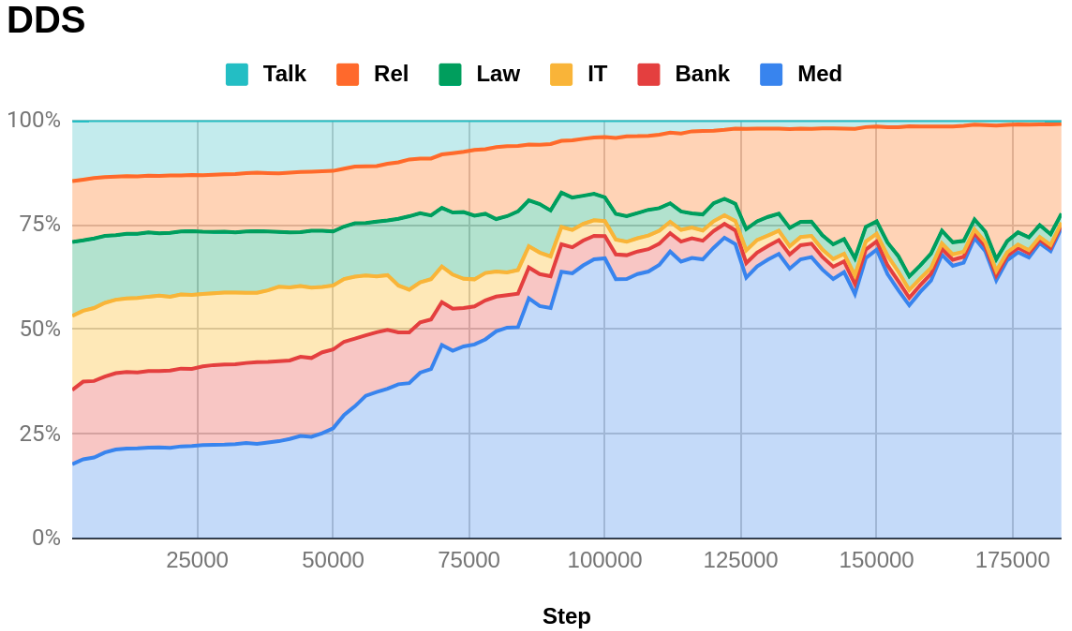
\includegraphics[width=.8\linewidth]{DDS.png}  
  \caption{DDS}
  \label{fig:DDS}
\end{subfigure}
\begin{subfigure}{.5\textwidth}
  \centering
  % include second image
  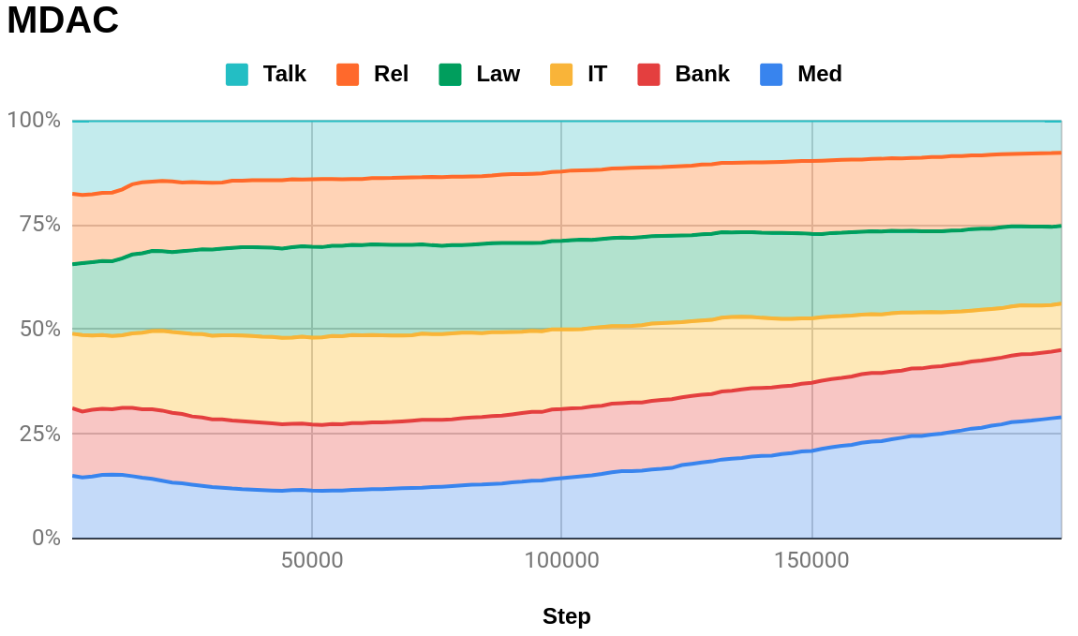
\includegraphics[width=.8\linewidth]{MDAC.png}  
  \caption{MDAC}
  \label{fig:MDAC}
\end{subfigure}
\caption{Sampling distribution}
\label{fig:sampling}
\end{figure*}

\subsection{Bi-domain adaptation}

\begin{table*}[htbp]
  \centering \small
  \begin{tabular}{|l|*9{r|}} \hline
    domain \hfill $d=$ & \multicolumn{1}{c|}{\domain{ med}} & \multicolumn{1}{c|}{\domain{ law}} & \multicolumn{1}{c|}{\domain{bank}} & \multicolumn{1}{c|}{\domain{talk}} & \multicolumn{1}{c|}{\domain{ it }} & \multicolumn{1}{c|}{\domain{ rel}} & \multicolumn{1}{c|}{mean} & \multicolumn{1}{|c|}{\domain{news}} \\ \hline \hline
    \system{MDAC($\vlambda_1, \vlambda_2$)}&36.2&-&-&-&46.1$^*$&-&-&- \\
    \system{DDS($\vlambda_1, \vlambda_2$)}&36.5&-&-&-&44.4&-&-&- \\
    \system{MDAC($\vlambda_1, \vlambda_2$)}&-&57.2$^*$&53.8$^*$&-&-&-&-&- \\
    \system{DDS($\vlambda_1, \vlambda_2$)}&-&56.1&52.6&-&-&-&-&- \\
    \system{MDAC($\vlambda_1, \vlambda_2$)}&-&-&-&32&-&90&-&- \\
    \system{DDS($\vlambda_1, \vlambda_2$)}&-&-&-&32.9&-&91.1&-&- \\ \hline
  \end{tabular}
  \caption{Non empty columns correspond to the target domains. For a given line, all the non empty columns \emph{correspond to the same bi-domain system}. ($^*$) MDAC is significantly better than DDS with $p<0.05$.}
  \label{tab:bi-da}
\end{table*}
According to Table \ref{tab:bi-da}, MDAC outperforms DDS in 2 over 3 settings including adapting to \domain{med-it} and \domain{law-bank} while being surpassed in \domain{talk-rel}, showing that MDAC is capable to adapt to a variable set of target domains.

\begin{table*}[htbp]
  \centering \small
  \begin{tabular}{|l|*9{r|}} \hline
    domain \hfill $d=$ & \multicolumn{1}{c|}{\domain{ med}} & \multicolumn{1}{c|}{\domain{ law}} & \multicolumn{1}{c|}{\domain{bank}} & \multicolumn{1}{c|}{\domain{talk}} & \multicolumn{1}{c|}{\domain{ it }} & \multicolumn{1}{c|}{\domain{ rel}} & \multicolumn{1}{c|}{mean} & \multicolumn{1}{|c|}{\domain{news}} \\ \hline \hline
    \multicolumn{9}{|c|}{\sl Unsupervised domain adaptation} \\ \hline
    \system{Mixed-0}      & - & - & - & - & - & - & - & 22.4 \\
    \system{Mixed-0.25} & - & - & - & - & - & - & - & 22.7\\
    \system{Mixed-0.5}   & - & - & - & - & - & - & - & 23.6\\
    \system{Mixed-0.75} & - & - & - & - & - & - & - & 23.7\\
    \system{Mixed-1} & - & - & - & - & - & - & - & 23.5\\
    \hline \hline
    \system{MDAC($\vlambda_0, \vlambda_{news}$)} &-&-&-&-&-&-&-&23.1 \\
     \system{DDS($\vlambda_0, \vlambda_{news}$)} &-&-&-&-&-&-&-&23.3 \\ \hline\hline 
    \multicolumn{9}{|c|}{\sl 30 clusters} \\ \hline
    \system{MDAC($\vlambda^*, \vlambda_d$)}&36.3$^*$&56.9$^*$&51.3$^*$&33.2$^*$&43.4&89.4&51.8$^*$&-\\
     \system{DDS($\vlambda^*, \vlambda_d$)}&35.3&55.2&49.4&30.6&43.3&89.9&50.6&-\\ \hline
  \end{tabular}
  \caption{Non empty columns correspond to the target domains. For a given line, each non empty column correspond to one expert system. ($^*$)MDAC is significantly better than DDS.}
  \label{tab:unsupervised-da}
\end{table*}

\subsection{Unseen domains}
The top of Table \ref{tab:unsupervised-da} displays the performance on the unseen domain \domain{news} for NMT systems trained with the mixtures $\lambda^l \in \big[ \lambda_0, \lambda_{0.25}, \lambda_{0.5}, \lambda_{0.75}, \lambda_{1.0}\big]$ and dynamic data selection MDAC and DDS. These systems have insignificant differences in BLEU, showing that dynamic mixture does not improve the robustness of the NMT system against unseen domains. However, the fact that the performance of MDAC and DDS is close to the best performance guarantees the harmlessness of these algorithms to the robustness of the NMT model.

\subsection{Automatic clustering}
The bottom of Table \ref{tab:unsupervised-da} shows the performance of NMT systems adapted to each domain in using 30 clusters instead of 6 domains. According to Table \ref{tab:unsupervised-da}, MDAC outperforms DDS on every domain, proving the efficacy of the method in this situation where no information of the domain is given a priori.

\section{Related Work \label{sec:related}}

Domain adaptation is an ancient and vexing problem that has been studied from many angles both for SMT and NMT. A survey of supervised and unsupervised DA for NMT is in \citet{Chu18asurvey}, where they distinguish between data-centric and model-centric DA, a view also adapted in the more recent review of \citet{Saunders21domain}. Our approach to DA in this paper clearly falls under the former category. We refer interested readers to these refrences, and do not discuss review DA any further.

Multi-domain adaptation (MDA) aims to develop systems that simultaneously bode well for several domains. Like for DA, techniques for supervised MDA typically combine one or several ingredients: (a) the specialization of data representations \citep{Kobus17domaincontrol} or of sub-networks \citep{Pham19generic} to differentiate the processing of each domain; (b) the use of adversarial techniques to neutralize differences between domains \cite{Britz17mixing,Zeng18multidomain}; (c) the use of automatic domain identification e.g.\ \citet{Jiang19multidomain}. Unsupervised MDA is considered in \citet{Farajian17multidomain} as an unsupervised DA problem.

Most approaches to adaptive / dynamic data selection take inspiration from \citet{Bengio09curriculum}, where the notion of \emph{curriculum learning} (CL) is initially introduced. CL is relies on a notion of ``easyness'' of a sample to schedule the presentation of the training data so that the easiest examples  presented first and the hardest, last. CL has been showed to speed up learning. While the initial aim was to improve and speed up training, it has also proven useful for domain adaptive / multi-domain / multi-lingual MT, based on alternative definitons of ``easyness''.

For instance, \citet{Zhang19curriculum} study supervised domain adaptation, and propose a curriculum approach which progressively extends the data used in training: in the early stages only in-data is used, while shards containing less relevant\footnote{Domain distance is computed with Lewis-Moore scores (based on the cross-entropy of in-domain LM).} data are introduced in later stages. This is somehow opposite to the recommendations of \citet{Vanderwees17dynamic}, whose \emph{gradual fine-tuning} progressively focuses on the in-domain data.\fyTodo{These have not been compared ? and also to what we do ?} 

\citet{Kumar19reinforcement} use reinforcement techniques (deep Q-learning) to learn the curriculum strategy: in this study, complexity corresponds to difficulty levels and which are binned based on contrastive data selection. The reward is based on the increase of the development set loss that results from the actual data selection strategy.\fyTodo{Alert: what do we do during warm up ?} The same technique is recently applied to the training of a multilingual NMT system \citep{Kumar21learning}. \citet{Zhou20uncertainty} propose another curriculum-based approach which instead relies on \emph{instance uncertainty} as a measure of their difficulty and presents the data sample starting with the easiest (more predictable) first. Another contribution of this paper is an alternative criterium for stopping the training. More related to our problems, \citet{Wang20learning-multi} adapt curriculum learning for multi-domain adaptation, where an optimal instance weighting scheme is found using Bayesian optimization (derivative-free) techniques. Each step consists in (a) weighting the instances based on relevance features, (b) fine tuning current model using the (weighted) training set, and is applied iteratively to generate a sequence of models. The one that maximizes the development set performance is finally retained.

\section*{Acknowledgments}
\bibliographystyle{acl_natbib}
\bibliography{multidomain}
%\appendix
\end{document}












